\documentclass{beamer}  
\usepackage{../slides}
\usepackage{cancel}
\usepackage{appendixnumberbeamer}
\setbeameroption{hide notes}
\defbeamertemplate{description item}{align left}{\insertdescriptionitem\hfill}

%%%%%%%%%%%%%%%%%%%% Not needed at home!
\usepackage[compatibility=false]{caption}
\usepackage{subcaption}
%%%%%%%%%%%%%%%%%%%% Not needed at home!


\title[Binary Regressors]{Estimating the Effect of a Mis-measured, Endogenous, Binary Treatment}
\author[FJ DiTraglia]{Francis J.\ DiTraglia\\ Camilo Garcia-Jimeno}
\institute{University of Pennsylvania}
\date{February 27th, 2017}
\begin{document} 
%%%%%%%%%%%%%%%%%%%%%%%%%%%%%%%%%%%%%%%%

\begin{frame}[plain]
	\titlepage 
\end{frame} 
%%%%%%%%%%%%%%%%%%%%%%%%%%%%%%%%%%%%%%%%%
\begin{frame}
  \frametitle{Estimating the Effect of $T^*$}
  \vspace{-1em}
  \[ y_i = h(T^*_i, \mathbf{x}_i) + \varepsilon_i\]
  \vspace{-1.5em}
  \begin{itemize}
    \item $y$ -- Outcome of interest
    \item $h$ -- Known or Unknown function 
    \item $T^*$ -- Unobserved, endogenous binary treatment
    \item $T$ -- Observed, mis-measured binary surrogate for $T^*$
    \item $\mathbf{x}$ -- Exogenous covariates
    \item $\varepsilon$ -- Mean-zero error term
    \item $z$ -- Discrete (typically binary) instrumental variable
  \end{itemize}

  \begin{block}{Target of Inference: $\tau(\mathbf{x}) = h(1,\mathbf{x}) - h(0,\mathbf{x})$}
  \end{block}
\end{frame}
%%%%%%%%%%%%%%%%%%%%%%%%%%%%%%%%%%%%%%%%%
\begin{frame}
  \frametitle{Example: Job Training Partnership Act (JPTA)}
\framesubtitle{Heckman et al.\ (2000, QJE)}
Randomized offer of job training, but about $30\%$ of those \emph{not} offered also obtain training and about $40\%$ of those offered training don't attend. Estimate causal effect of \emph{training} rather than \emph{offer} of training.

\begin{itemize}
  \item $y$ -- Log wage 
  \item $T^*$ -- True training attendence
  \item $T$ -- Self-reported training attendance
  \item $\mathbf{x}$ -- Individual characteristics
  \item $z$ -- Offer of job training
\end{itemize}
   
\end{frame}
%%%%%%%%%%%%%%%%%%%%%%%%%%%%%%%%%%%%%%%%%%%%
%\begin{frame}
%  \frametitle{Example: Smoking and Birthweight (SNAP Trial)}
%\framesubtitle{Coleman et al.\ (N Engl J Med, 2012)}
%  RCT with 1050 pregnant smokers in England: 521 given nicotine patches, the rest given placebo patches.
%\begin{itemize}
%  \item $y$ -- Birthweight 
%  \item $T^*$ -- True smoking behavior 
%  \item $T$ -- Self-reported smoking behavior
%  \item $\mathbf{x}$ -- Mother characteristics
%  \item $z$ -- Indicator of nicotine patch
%\end{itemize}
%   
%\end{frame}
%%%%%%%%%%%%%%%%%%%%%%%%%%%%%%%%%%%%%%%%%%
%\begin{frame}
%  \frametitle{Example: Schooling and Test Scores}
%\framesubtitle{Burde \& Linden (2013, AEJ Applied)}
%  RCT in Afghanistan: 32 villages divided into 11 clusters. Randomly choose 6 and set up school in each village of these clusters.
%
%\begin{itemize}
%  \item $y$ -- Girl's score on math and language test 
%  \item $T^*$ -- Girl's true school attendance
%  \item $T$ -- Parent's report of child's school attendance
%  \item $\mathbf{x}$ -- Child and household characteristics
%  \item $z$ -- School built in village
%\end{itemize}
%\end{frame}
%%%%%%%%%%%%%%%%%%%%%%%%%%%%%%%%%%%%%%%%%%%
%\begin{frame}
%  \frametitle{Example: Returns to Schooling} 
%\framesubtitle{Oreopoulos (2006, AER)}
%Fuzzy RD: minimum school-leaving age in UK increased from 14 to 15 in 1947 but some already stayed until 15 before the law and others failed to comply after it.
%\begin{itemize}
%  \item $y$ -- Log wage 
%  \item $T^*$ -- School attendance at age 15
%  \item $T$ -- Self-report of school attendance at age 15
%  \item $\mathbf{x}$ -- Individual characteristics
%  \item $z$ -- Indicator: born in or after 1933
%\end{itemize}
%   
%\end{frame}
%%%%%%%%%%%%%%%%%%%%%%%%%%%%%%%%%%%%%%%%%%%
\begin{frame}[label=MAHAJAN_BODY]
  \frametitle{Related Literature}
 
  \begin{block}{Continuous Treatment}
    \small
  Lewbel (1997, 2012), Schennach (2004, 2007), Chen et al. (2005), Hu \& Schennach (2008), Song (2015), Hu et al.\ (2015)\ldots 
  \end{block}

  \begin{block}{Binary, Exogenous Treatment}
    \small
   Aigner (1973), Bollinger (1996), Kane et al. (1999), Black et al. (2000), Frazis \& Loewenstein (2003), Mahajan (2006), Lewbel (2007) 
  \end{block}

  \begin{block}{Binary, Endogenous Treatment}
    \alert{Mahajan (2006)}, \small Shiu (2015), Ura (2015), Denteh et al.\ (2016)  
  \end{block}
    \hyperlink{MAHAJAN_APPEND}{\beamergotobutton{Mahajan Details}}
\end{frame}
%%%%%%%%%%%%%%%%%%%%%%%%%%%%%%%%%%%%%%%
%\begin{frame}
%  \frametitle{Model: $y = h(T^*, \mathbf{x}) + \varepsilon$}
%  \begin{block}{ATE Function}
%   $ \tau(\mathbf{x}) = h(1,\mathbf{x}) - h(0, \mathbf{x})$
%  \end{block}
%  \begin{block}{First-stage}
%    $p^*_k(\mathbf{x}) \equiv \mathbb{P}(T^*=1|z=z_k,\mathbf{x}) \neq \mathbb{P}(T^*=1|z=z_\ell, \mathbf{x})\equiv p_\ell^*(\mathbf{x}) $, $k\neq \ell$
%  \end{block}
%  \begin{block}{Measurement Error}
%    Non-differential, $\mathbb{E}[\varepsilon|T^*,T,z,\mathbf{x}] =  \mathbb{E}[\varepsilon|T^*,z,\mathbf{x}]$, and does not depend on $z$:
%\begin{eqnarray*}
% \alpha_0(\mathbf{x})&=&  \mathbb{P}(T = 1| T^* = 0, z, \mathbf{x})  \\ 
% \alpha_1(\mathbf{x})&=& 
%  \mathbb{P}(T = 0| T^* = 1, z, \mathbf{x}) 
%\end{eqnarray*}
%    
%  \end{block}
%\end{frame}
%%%%%%%%%%%%%%%%%%%%%%%%%%%%%%%%%%%%%%%
%\begin{frame}
%  \frametitle{Notation}
%
%  \begin{itemize}
%    \item Treat exog.\ covariates $\mathbf{x}$ non-parametrically: hold fixed at $\mathbf{x}_a$ throughout:
%      \vspace{-1em}
%      \begin{eqnarray*}
%        y &=&  \beta T^* + u\\
%        u &=&  \varepsilon + c
%      \end{eqnarray*}
%      where $\beta = \tau(\mathbf{x}_a)$ and $c = h(0,\mathbf{x}_a)$.
%    \item Similarly:
%      \begin{eqnarray*}
%        \alpha_0 &=&  \mathbb{P}(T=1|T^*=0)\\
%        \alpha_1 &=&  \mathbb{P}(T=0|T^*=1)\\
%        p_k^* &=&  \mathbb{P}(T^* = 1|z=z_k)
%      \end{eqnarray*}
%  \end{itemize}
%\end{frame}
%%%%%%%%%%%%%%%%%%%%%%%%%%%%%%%%%%%%%%%
\begin{frame}
  \frametitle{Model: $y = c + \beta T^* + \varepsilon$}

  \begin{block}{Valid Instrument}
    $\mathbb{E}[\varepsilon|z] =0$. 
  \end{block}

  \begin{block}{First-stage}
    $p^*_k \equiv \mathbb{P}(T^*=1|z=z_k) \neq \mathbb{P}(T^*=1|z=z_\ell)\equiv p_\ell^*$, $k\neq \ell$
  \end{block}

  \begin{block}{Non-differential Measurement Error}
    \begin{itemize}
      \item $\mathbb{E}[\varepsilon|T^*,T,z] =  \mathbb{E}[\varepsilon|T^*,z]$
      \item $\alpha_0 = \mathbb{P}(T = 1| T^* = 0, z)$ 
      \item  $\alpha_1 = \mathbb{P}(T = 0| T^* = 1, z)$ 
      \item $\alpha_0 + \alpha_1 < 1$ 
    \end{itemize}
  \end{block}


\end{frame}
%%%%%%%%%%%%%%%%%%%%%%%%%%%%%%%%%%%%%%
\begin{frame}
  \frametitle{Observable Moments:  $y = c + \beta T^* + \varepsilon$}

\phantom{Define error term that absorbs constant: $u = c + \varepsilon$}

\begin{center}
  \begin{tabular}{c|c|c|c|c|}
    \multicolumn{1}{c}{}& \multicolumn{1}{c}{$z=1$} &\multicolumn{1}{c}{$z=2$} & \multicolumn{1}{c}{\dots} &\multicolumn{1}{c}{$z=K$}\\
    \cline{2-5}
    $T=0$ & \diagbox[dir=NE]{$\bar{y}_{01}$}{$p_{01}$} & \diagbox[dir=NE]{$\bar{y}_{02}$}{$p_{02}$} & \dots &\diagbox[dir=NE]{$\bar{y}_{0K}$}{$p_{0K}$}\\
    \cline{2-5}
    $T=1$ & \diagbox[dir=NE]{$\bar{y}_{11}$}{$p_{11}$} & \diagbox[dir=NE]{$\bar{y}_{12}$}{$p_{12}$} & \dots &\diagbox[dir=NE]{$\bar{y}_{1K}$}{$p_{1K}$}\\
    \cline{2-5}
  \end{tabular}
\end{center}

\vspace{1em}

\[\bar{y}_{tk} = \mathbb{E}[y|T=t,z=z_k],
\quad p_{tk} =q_k p_k\]
\small
\[q_k = \mathbb{P}(z = z_k), \quad
p_k = \mathbb{P}(T=1|z=z_k)\]

\end{frame}

%%%%%%%%%%%%%%%%%%%%%%%%%%%%%%%%%%%%%%
\begin{frame}
  \frametitle{Unobservable Moments: $y = \beta T^* + u$}

\alert{Define error term that absorbs constant: $u = c + \varepsilon$}

\begin{center}
  \begin{tabular}{c|c|c|c|c|}
    \multicolumn{1}{c}{}& \multicolumn{1}{c}{$z=1$} &\multicolumn{1}{c}{$z=2$} & \multicolumn{1}{c}{\dots} &\multicolumn{1}{c}{$z=K$}\\
    \cline{2-5}
    $T^*=0$ & \diagbox[dir=NE]{$m^*_{01}$}{$p^*_{01}$} & \diagbox[dir=NE]{$m^*_{02}$}{$p^*_{02}$} & \dots &\diagbox[dir=NE]{$m^*_{0K}$}{$p^*_{0K}$}\\
    \cline{2-5}
    $T^*=1$ & \diagbox[dir=NE]{$m^*_{11}$}{$p^*_{11}$} & \diagbox[dir=NE]{$m^*_{12}$}{$p^*_{12}$} & \dots &\diagbox[dir=NE]{$m^*_{1K}$}{$p^*_{1K}$}\\
    \cline{2-5}
  \end{tabular}
\end{center}

\vspace{1em}

\[m^*_{tk} = \mathbb{E}[u|T^*=t,z=z_k],
\quad p^*_{tk}=q_k p^*_k\]
\small
\[q_k = \mathbb{P}(z = z_k),\quad p^*_k=\mathbb{P}(T^*=1|z=z_k)\]

\end{frame}
%%%%%%%%%%%%%%%%%%%%%%%%%%%%%%%%%%%%%%
%\begin{frame}
%  \frametitle{Unrestricted System of Equations} 
%  \begin{eqnarray*}
%   (1 - p_k) \bar{y}_{0k} &\equiv& \alert{\widetilde{y}_{0k}= (\beta + m_{1k}^*) \alpha_1 p_k^*  + (1 -\alpha_0)(1 - p^*_k)m_{0k}^* } \\
%    p_k \bar{y}_{1k} &\equiv&  \alert{\widetilde{y}_{1k}=(\beta + m_{1k}^*) (1 - \alpha_1)p_k^* + \alpha_0 (1 - p_k^*) m_{0k}^*} 
%  \end{eqnarray*}
%  \small
%  \[p^*_k =  \frac{p_k - \alpha_0}{1 - \alpha_0 - \alpha_1} \]
%
%\end{frame}
%%%%%%%%%%%%%%%%%%%%%%%%%%%%%%%%%%%%%%
%\begin{frame}
%  \frametitle{Possible Restrictions On $m^*_{tk}$}
%  \begin{block}{Joint Exogeneity: $\mathbb{E}[\varepsilon|T^*,z]=0$}
%    $\implies m^*_{tk} =c \quad$ for all $t,k$
%  \end{block}
%  \begin{block}{Exogenous Treatment: $\mathbb{E}[\varepsilon|T^*]=0$}
%    $\implies \displaystyle \frac{1}{\mathbb{P}(T^*=t)}\sum_{k}p^*_{tk}m^*_{tk} = c\quad$  for all $t$
%  \end{block}
%  \begin{alertblock}{Exogenous Instrument: $\mathbb{E}[\varepsilon|z]=0$}
%    $\implies (1-p^*_k)m^*_{0k} + p^*_k m^*_{1k}=c \quad$ for all $k$
%  \end{alertblock}
%
%\end{frame}
%%%%%%%%%%%%%%%%%%%%%%%%%%%%%%%%%%%%%%
\begin{frame}
  \frametitle{System of Equations given $E[\varepsilon|z]=0$}
  \small
  \alert{\framebox{$\mathbb{E}[\varepsilon|z]=0 \implies$ \emph{pair} of equations for each $k = 1, \dots, K$}}
\begin{align*}
  (1 - p_k)\bar{y}_{0k} &=\alpha_1(p_k - \alpha_0)\left(\frac{\beta}{1 - \alpha_0 - \alpha_1}\right) + (1-\alpha_0)c - (p _k -  \alpha_0)m_{1k}^* \\[1.5ex]
  p_k\bar{y}_{1k} &=(1-\alpha_1)(p_k - \alpha_0)\left(\frac{\beta}{1 - \alpha_0 - \alpha_1}\right) + \alpha_0 c + (p _k -  \alpha_0)m_{1k}^*
\end{align*}

\begin{alertblock}{Theorem}
  $2K$ equations in $K+4$ unknowns, but $\beta$ is unidentified \emph{regardless} of $K$.
\end{alertblock}

\begin{block}{Intuition}
  Using $E[\varepsilon|z]=0$ to eliminate $m_{0k}^*$ from the system ``entangles'' the equations such that each pair only provides one restriction.
\end{block}

\end{frame}
%%%%%%%%%%%%%%%%%%%%%%%%%%%%%%%%%%%%%%%%%%%%%%%%%%
%\begin{frame}
%  \frametitle{Sufficient Conditions To Identify $\alpha_0, \alpha_1$, and $\beta$}
%  \small
%
%  \begin{block}{Baseline Assumptions}
%  \vspace{-1em}
%    \begin{itemize}
%      \item $\mathbb{E}[\varepsilon|z] =0$
%      \item $\mathbb{E}[\varepsilon|T^*,T,z] = \mathbb{E}[\varepsilon|T^*,z]$
%      \item $\alpha_0 = \mathbb{P}(T=1|T^*=0,z), \; \alpha_1 =\mathbb{P}(T=0|T^*=1, z), \; \alpha_0 + \alpha_1 < 1$
%    \end{itemize}
%  \end{block}
%
%  \vspace{-1em}
%  
%  \begin{alertblock}{Strengthen IV Assumption}
%  \vspace{-1em}
%    \begin{itemize}
%      \item $\mathbb{E}[\varepsilon^2|z] = \mathbb{E}[\varepsilon^2]$  
%      \item $\mathbb{E}[\varepsilon^3|z] = \mathbb{E}[\varepsilon^3]$  
%    \end{itemize}
%  \end{alertblock}
%
%  \vspace{-1em}
%  \begin{alertblock}{Strengthen Measurement Error Assumption}
%  \vspace{-1em}
%    \begin{itemize}
%      \item $\mathbb{E}[\varepsilon^2|T^*,T,z] = \mathbb{E}[\varepsilon^2|T^*,z]$  
%      \item $\mathbb{E}[\varepsilon^3|T^*,T,z] = \mathbb{E}[\varepsilon^3|T^*,z]$  
%    \end{itemize}
%
%  \end{alertblock}
%
%\end{frame}
%%%%%%%%%%%%%%%%%%%%%%%%%%%%%%%%%%%%%%
\begin{frame}
  \frametitle{First Moment Condition}
  \begin{block}{Assumptions}
    \begin{itemize}
      \item $\mathbb{E}[\varepsilon|z]=0$
      \item $\mathbb{E}[\varepsilon|T^*,T,z] =  \mathbb{E}[\varepsilon|T^*,z]$
      \item $\alpha_0 = \mathbb{P}(T = 1| T^* = 0, z)$ 
      \item  $\alpha_1 = \mathbb{P}(T = 0| T^* = 1, z)$ 
    \end{itemize}
  \end{block}

  \begin{block}{Moment Condition}
    \[\mbox{Cov}(y,z) - \left( \frac{\beta}{1 - \alpha_0 - \alpha_1} \right) \mbox{Cov}(T,z) = 0\]
  \end{block}

  \alert{MC \# 1 identifies $\beta/(1 - \alpha_0 - \alpha_1)$}
\end{frame}
%%%%%%%%%%%%%%%%%%%%%%%%%%%%%%%%%%%%%%
\begin{frame}
  \frametitle{Second Moment Condition}
  \begin{block}{Additional Assumptions}
    \begin{itemize}
      \item $\mathbb{E}[\varepsilon^2|z]=\mathbb{E}[\varepsilon^2]$
      \item $\mathbb{E}[\varepsilon^2|T^*,T,z] =  \mathbb{E}[\varepsilon^2|T^*,z]$
    \end{itemize}
  \end{block}

  \begin{block}{Moment Condition}
    \small
  \[\mbox{Cov}(y^2,z) - \frac{\beta}{1 - \alpha_0 - \alpha_1}\left\{2\mbox{Cov}(yT,z)- \beta \mbox{Cov}(T,z)\left( \frac{1 + \alpha_0 - \alpha_1}{1 - \alpha_0 - \alpha_1} \right)  \right\} = 0\]
  \end{block}

  \alert{Given MC \#1, MC \#2 identifies $(\alpha_1 - \alpha_0)$}
\end{frame}
%%%%%%%%%%%%%%%%%%%%%%%%%%%%%%%%%%%%%%
\begin{frame}
  \frametitle{Third Moment Condition}
  \begin{block}{Additional Assumptions}
    \begin{itemize}
      \item $\mathbb{E}[\varepsilon^3|z]=\mathbb{E}[\varepsilon^3]$
      \item $\mathbb{E}[\varepsilon^3|T^*,T,z] =  \mathbb{E}[\varepsilon^3|T^*,z]$
    \end{itemize}
  \end{block}
  \begin{block}{Moment Condition}
\scriptsize
\begin{align*}
  \mbox{Cov}(y^3,z) - \left( \frac{\beta}{1 - \alpha_0 - \alpha_1} \right)\Bigg \{& \left. \beta^2\left[1 + \frac{6\alpha_0(1 - \alpha_1)}{(1 - \alpha_0 - \alpha_1)^2} \right] \mbox{Cov}(T,z)\right.\\ & \left. - 3\beta\left[ \frac{1 - (\alpha_1 - \alpha_0)}{1 - \alpha_0 - \alpha_1} \right] \mbox{Cov}(yT,z) + 3\mbox{Cov}(y^2T,z) \right\} = 0
\end{align*}
\end{block}
\normalsize
\begin{alertblock}{Theorem}
  Third moment suffice to identify the model provided that $\beta \neq 0$. If $\beta = 0$, the reduced form identifies $\beta$.
\end{alertblock}
\end{frame}
%%%%%%%%%%%%%%%%%%%%%%%%%%%%%%%%%%%%%%
\begin{frame}
  \frametitle{GMM Estimator in Simple Special Case: $\alpha_0 = 0$}

  \vspace{-2em}

\begin{align*}
  u(\boldsymbol{\theta}) &= y - c - \frac{\beta}{1 - \alpha_1} T\\
  v(\boldsymbol{\theta}) &= y^2 - \sigma_{\varepsilon\varepsilon} - c^2 - \frac{\beta}{1 - \alpha_1} 2yT + \frac{\beta^2}{1 - \alpha_1}
\end{align*}

\vspace{-1em}

\[
  \mathbb{E}\left[ g_1(\mathbf{x}, \boldsymbol{\theta}) \right] = \mathbb{E}
  \left[
  \begin{array}{c}
    u(\boldsymbol{\theta})\\ v(\boldsymbol{\theta})
  \end{array}
\right] = \mathbf{0}, \quad
\mathbb{E}\left[ g_2(\mathbf{x}, \boldsymbol{\theta}) \right] = \mathbb{E}
  \left[
  \begin{array}{c}
    u(\boldsymbol{\theta}) z\\ v(\boldsymbol{\theta}) z
  \end{array}
\right] = \mathbf{0}
\]

  \[
    \alert{\beta = \frac{2\mbox{Cov}(yT,z)}{\mbox{Cov}(T,z)} - \frac{\mbox{Cov}(y^2,z)}{\mbox{Cov}(y,z)}}
  \]

\end{frame}
%%%%%%%%%%%%%%%%%%%%%%%%%%%%%%%%%%%%%%
%%%%%%%%%%%%%%%%%%%%%%%%%%%%%%%%%%%%%%
\begin{frame}
  \frametitle{Simulation DGP: $y = \beta T^* + \varepsilon$}
  \begin{block}{Errors}
      $(\varepsilon, \eta) \sim $ jointly normal, mean 0, variance 1, correlation 0.5.
  \end{block}
  \begin{block}{First-Stage}
      \begin{itemize}
        \item Half of subjects have $z=1$, the rest have $z=0$.
        \item $T^* = \mathbf{1}\left\{ \gamma_0 + \gamma_1 z + \eta > 0 \right\}$
        \item $\delta = \mathbb{P}(T^* = 0|z =1) = \mathbb{P}(T^*=1|z=0)$
          %\begin{itemize}
        %\item $\gamma_0 = \Phi^{-1}(\delta)$
        %\item $\gamma_1 = \Phi^{-1}(1-\delta) - \Phi(\delta)$   
      %\end{itemize}
      \end{itemize}
  \end{block}
  \vspace{-1em}


  \begin{block}{Mis-classification}
      \begin{itemize}
        \item Set $\alpha_0 = 0$ 
        \item $T|T^*=1 \sim \mbox{Bernoulli}(1-\alpha_1)$
      \end{itemize}
  \end{block}
  
\end{frame}
%%%%%%%%%%%%%%%%%%%%%%%%%%%%%%%%%%%%%%
\begin{frame}[plain,c]

  \begin{figure}[h]
    \centering
    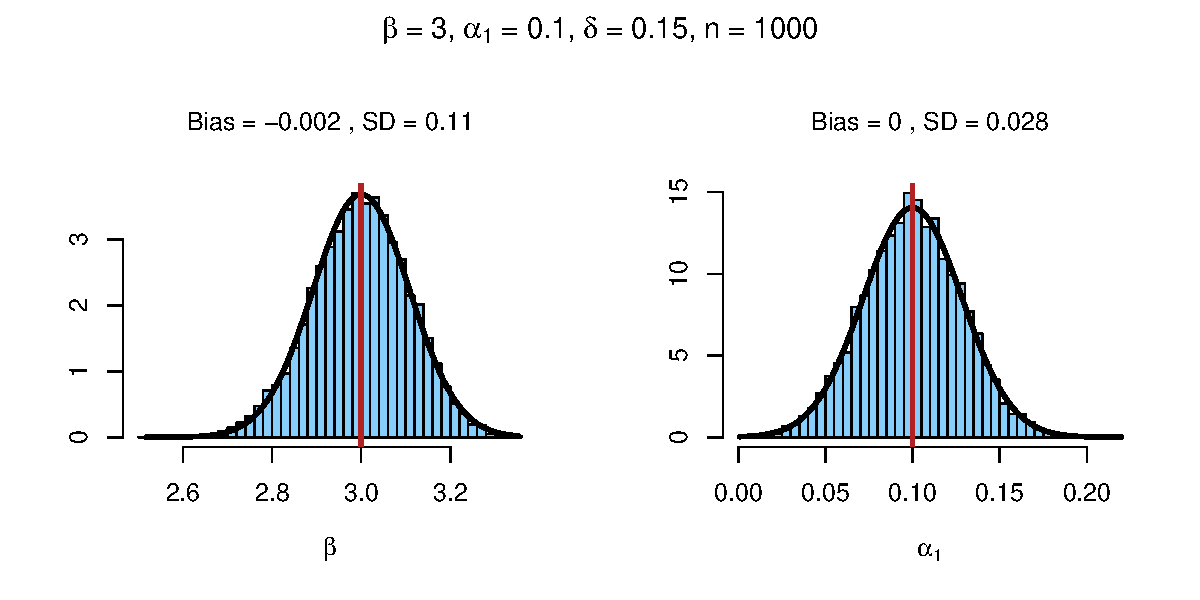
\includegraphics[width=\textwidth]{Rplot1}
  \end{figure}

\end{frame}
%%%%%%%%%%%%%%%%%%%%%%%%%%%%%%%%%%%%%%
\begin{frame}[plain,c]

  \begin{figure}[h]
    \centering
    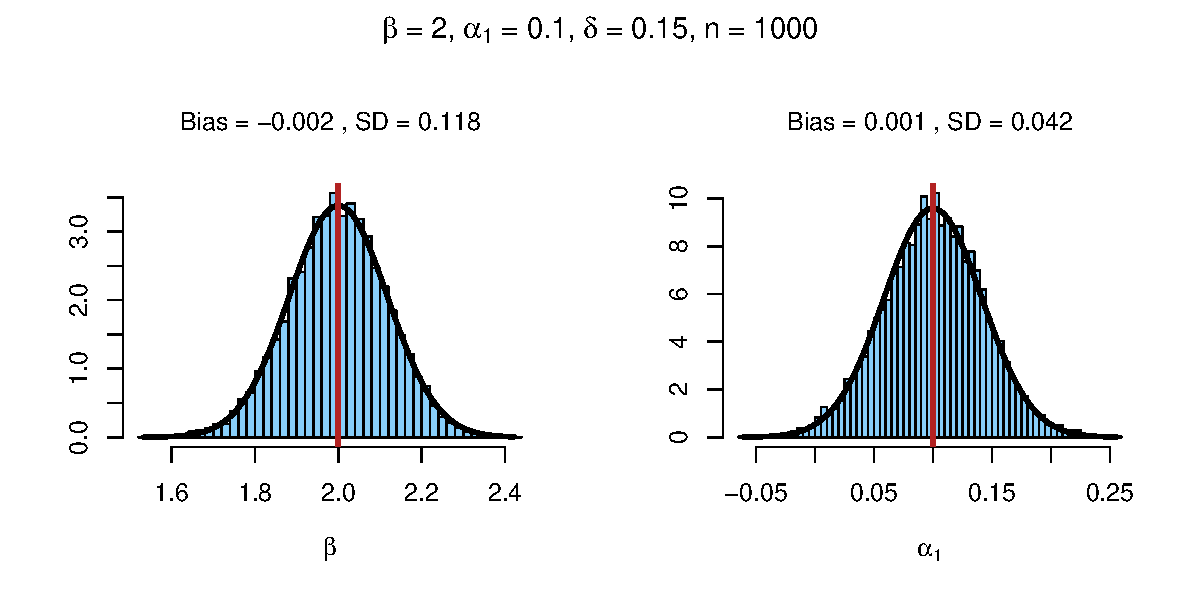
\includegraphics[width=\textwidth]{Rplot2}
  \end{figure}

\end{frame}
%%%%%%%%%%%%%%%%%%%%%%%%%%%%%%%%%%%%%%
\begin{frame}[plain,c]

  \begin{figure}[h]
    \centering
    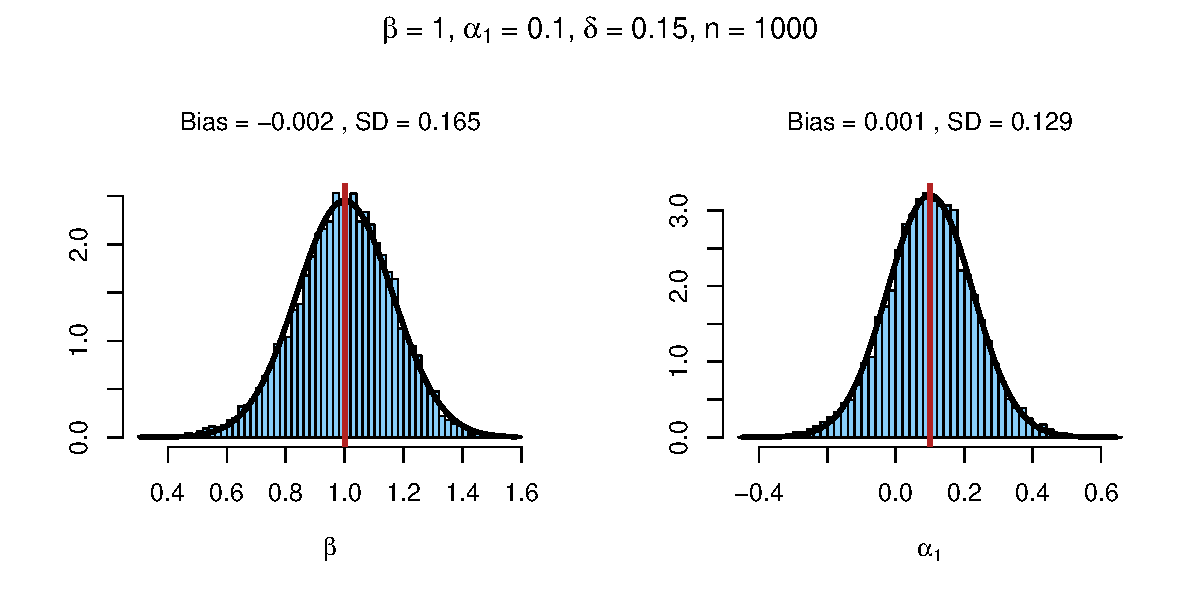
\includegraphics[width=\textwidth]{Rplot4}
  \end{figure}

\end{frame}
%%%%%%%%%%%%%%%%%%%%%%%%%%%%%%%%%%%%%%
%\begin{frame}[plain,c]
%
%  \begin{figure}[h]
%    \centering
%    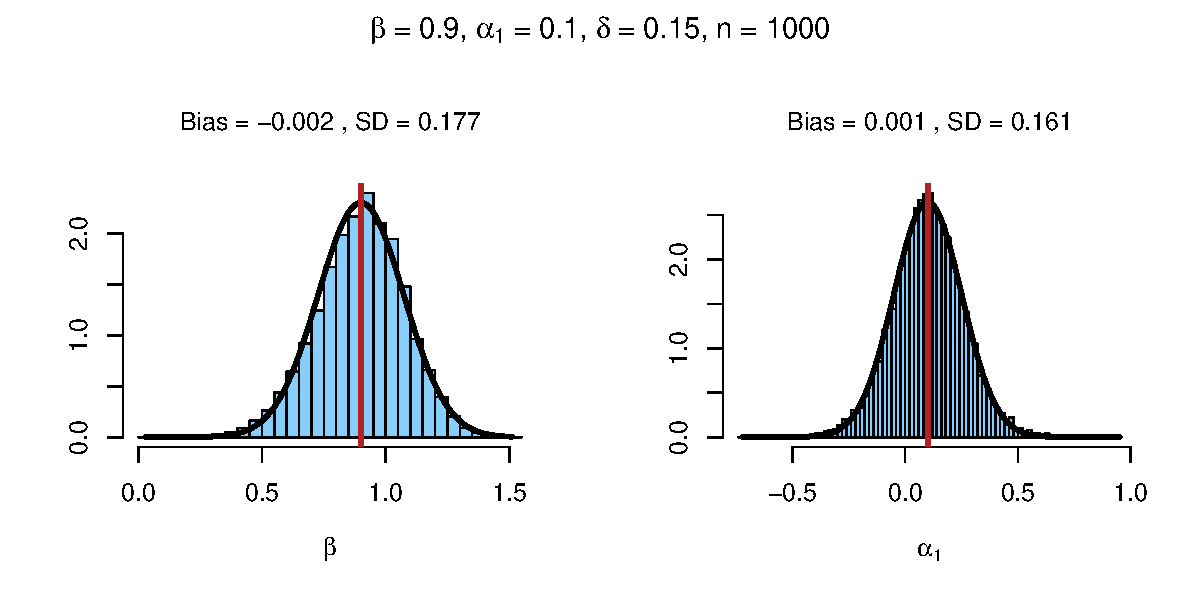
\includegraphics[width=\textwidth]{Rplot5}
%  \end{figure}
%
%\end{frame}
%%%%%%%%%%%%%%%%%%%%%%%%%%%%%%%%%%%%%%%%
%\begin{frame}[plain,c]
%
%  \begin{figure}[h]
%    \centering
%    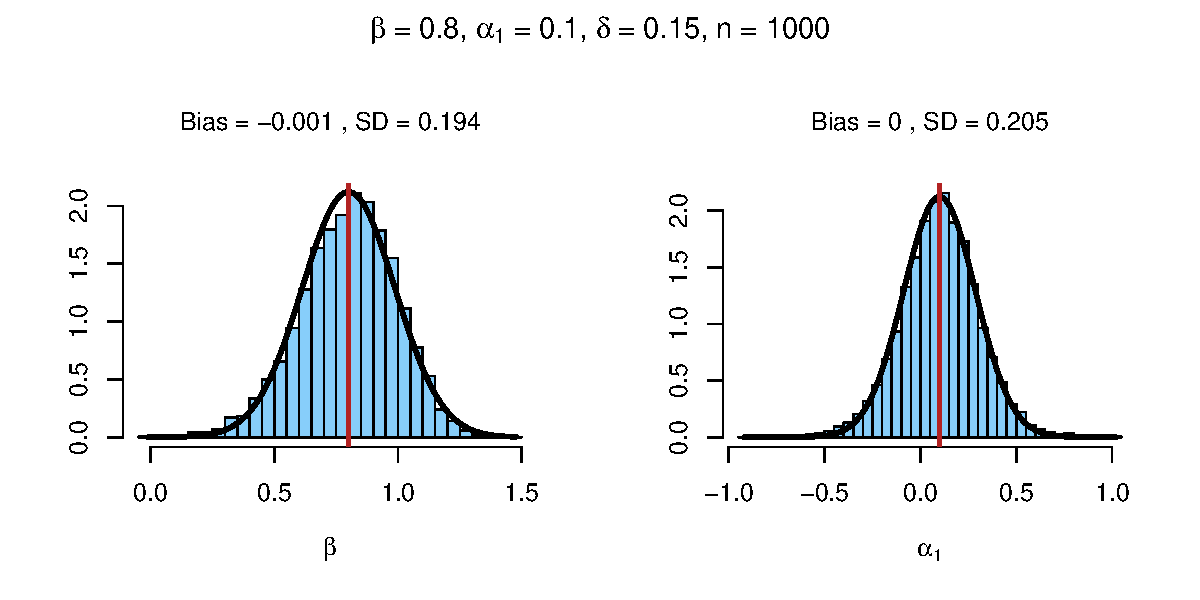
\includegraphics[width=\textwidth]{Rplot6}
%  \end{figure}
%
%\end{frame}
%%%%%%%%%%%%%%%%%%%%%%%%%%%%%%%%%%%%%%%
%\begin{frame}[plain,c]
%
%  \begin{figure}[h]
%    \centering
%    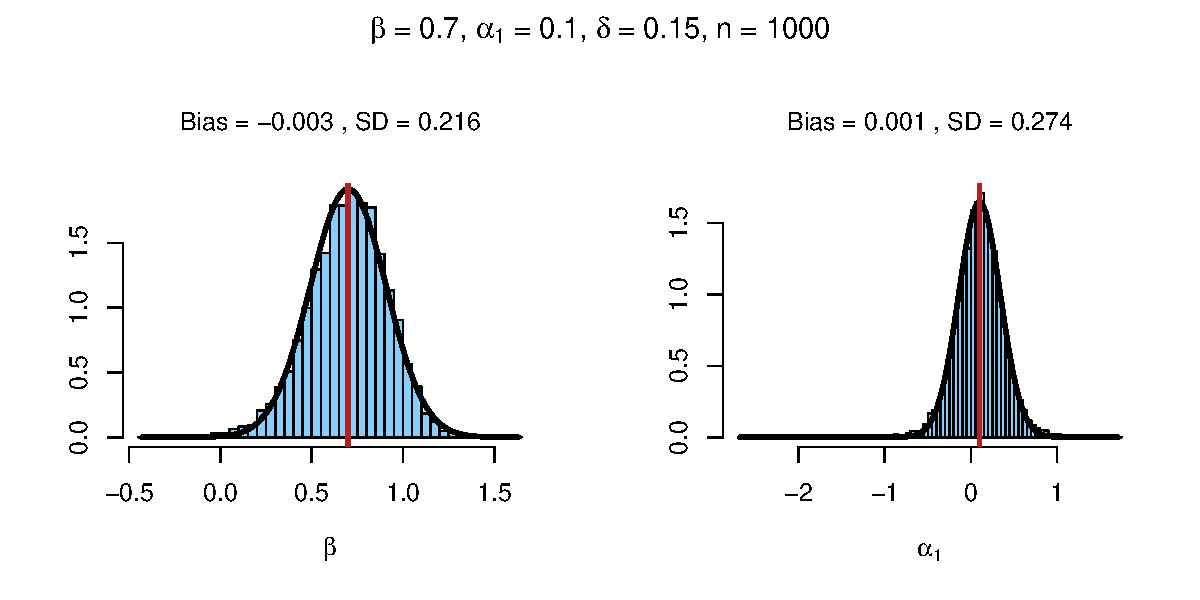
\includegraphics[width=\textwidth]{Rplot7}
%  \end{figure}
%
%\end{frame}
%%%%%%%%%%%%%%%%%%%%%%%%%%%%%%%%%%%%%%%%
%\begin{frame}[plain,c]
%
%  \begin{figure}[h]
%    \centering
%    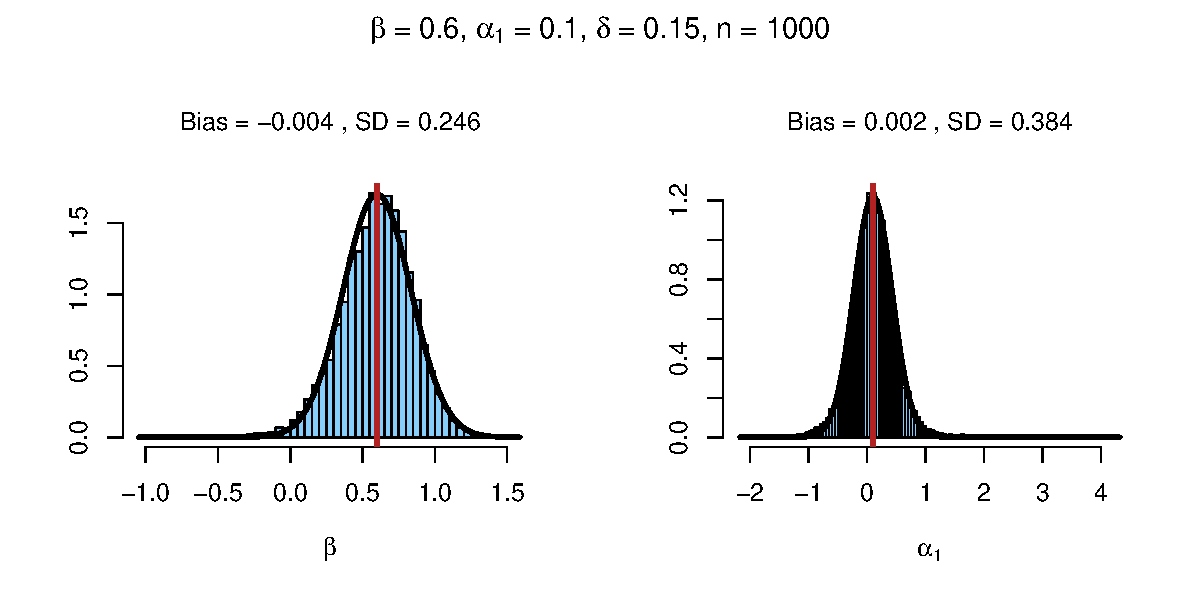
\includegraphics[width=\textwidth]{Rplot8}
%  \end{figure}
%
%\end{frame}
%%%%%%%%%%%%%%%%%%%%%%%%%%%%%%%%%%%%%%%
\begin{frame}[plain,c]

  \begin{figure}[h]
    \centering
    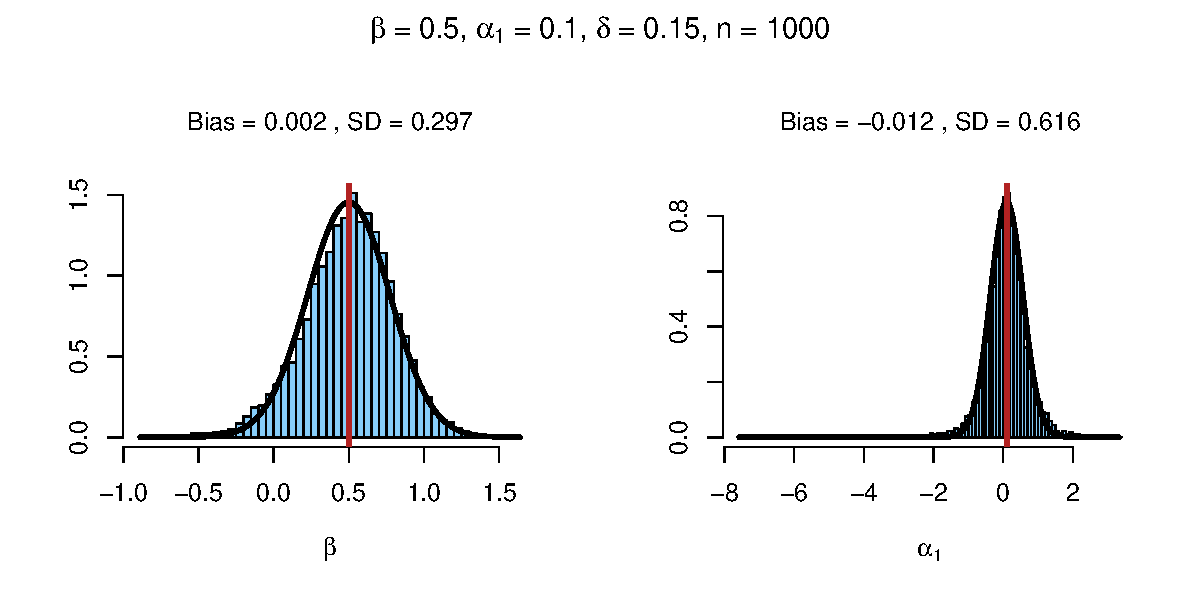
\includegraphics[width=\textwidth]{Rplot9}
  \end{figure}

\end{frame}
%%%%%%%%%%%%%%%%%%%%%%%%%%%%%%%%%%%%%%
%\begin{frame}[plain,c]
%
%  \begin{figure}[h]
%    \centering
%    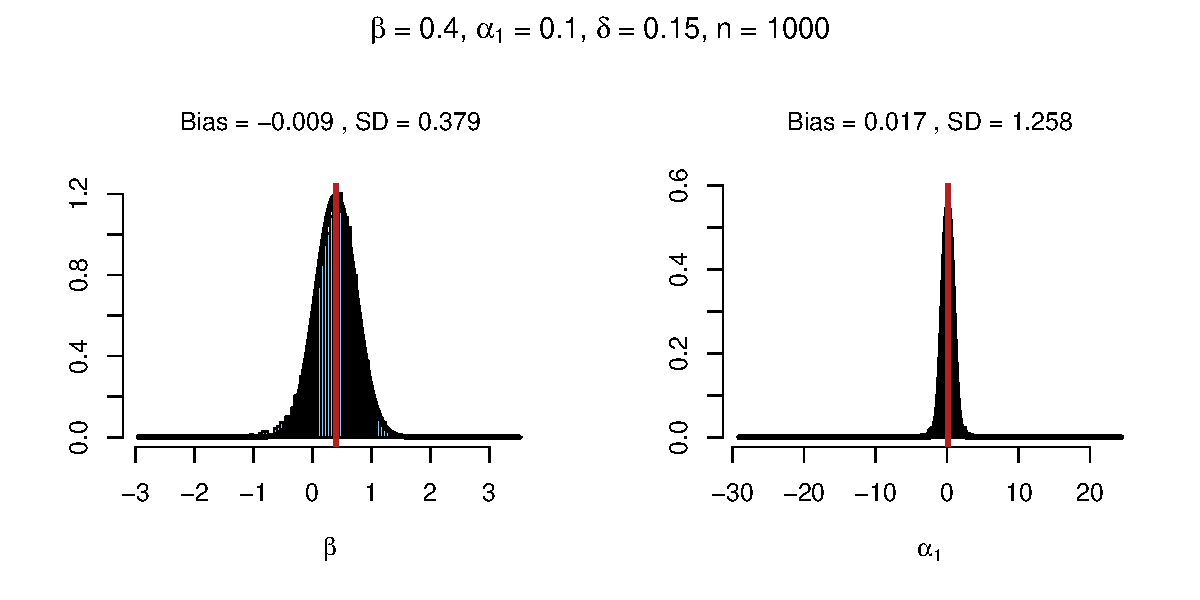
\includegraphics[width=\textwidth]{Rplot10}
%  \end{figure}
%
%\end{frame}
%%%%%%%%%%%%%%%%%%%%%%%%%%%%%%%%%%%%%%
%\begin{frame}[plain,c]
%
%  \begin{figure}[h]
%    \centering
%    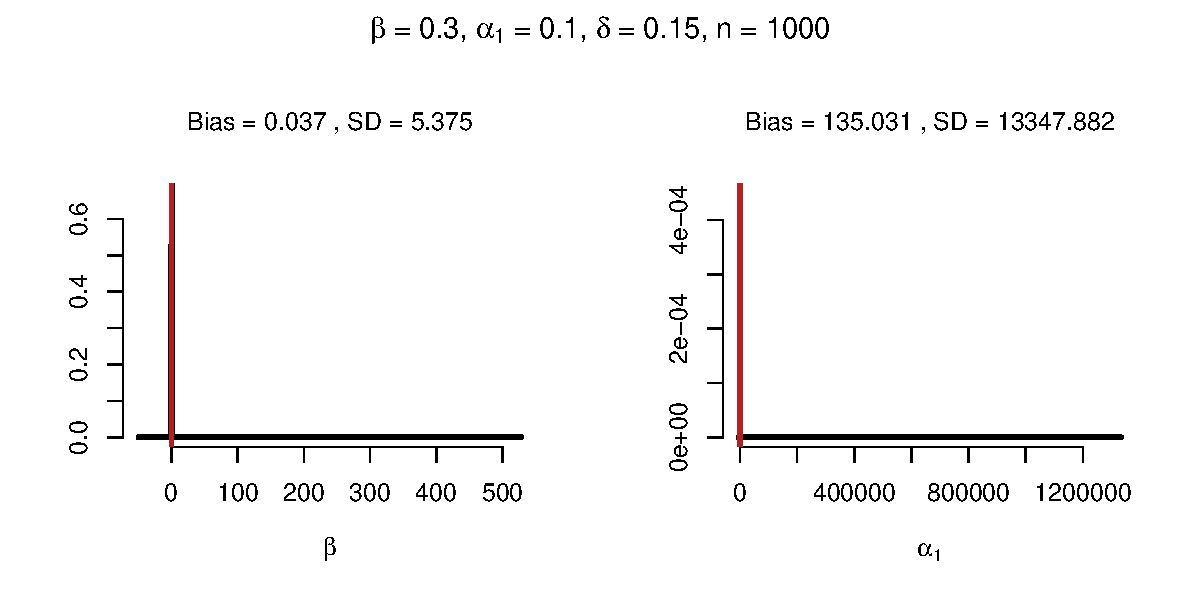
\includegraphics[width=\textwidth]{Rplot11}
%  \end{figure}
%
%\end{frame}
%%%%%%%%%%%%%%%%%%%%%%%%%%%%%%%%%%%%%%
%\begin{frame}
%  \frametitle{Coverage and Width of Nominal 95\% CIs}
%  \framesubtitle{$\alpha_1 = 0.1, \delta = 0.15, n = 1000, \rho = 0.5$}
%\begin{table}[!tbp]
%  \small
%\centering
%\begin{tabular}{rrrrrr}
%\hline\hline
%&& \multicolumn{2}{c}{Coverage} & \multicolumn{2}{c}{Width}\\
%\multicolumn{1}{c}{$\beta$}&\multicolumn{1}{c}{RF}&\multicolumn{1}{c}{RF}&\multicolumn{1}{c}{GMM}&\multicolumn{1}{c}{RF}&\multicolumn{1}{c}{GMM}\tabularnewline
%\hline
%$2.00$&$1.400$&$0.95$&$0.95$&$0.35$&$0.23$\tabularnewline
%$1.50$&$1.050$&$0.95$&$0.95$&$0.32$&$0.26$\tabularnewline
%$1.00$&$0.700$&$0.95$&$0.95$&$0.29$&$0.32$\tabularnewline
%$0.50$&$0.350$&$0.95$&$0.96$&$0.27$&$0.55$\tabularnewline
%$0.25$&$0.175$&$0.95$&$0.98$&$0.26$&$1.08$\tabularnewline
%$0.20$&$0.140$&$0.95$&$0.99$&$0.25$&$1.40$\tabularnewline
%$0.15$&$0.105$&$0.95$&$0.99$&$0.25$&$1.86$\tabularnewline
%$0.10$&$0.070$&$0.95$&$1.00$&$0.25$&$3.04$\tabularnewline
%$0.05$&$0.035$&$0.95$&$1.00$&$0.25$&$4.76$\tabularnewline
%$0.01$&$0.007$&$0.95$&$1.00$&$0.25$&$5.92$\tabularnewline
%\hline
%\end{tabular}
%\end{table}
%\end{frame}
%
%%%%%%%%%%%%%%%%%%%%%%%%%%%%%%%%%%%%%%
\begin{frame}
  \frametitle{Identification Failure when $\beta= 0$}
\framesubtitle{Simple Special Case: $\alpha_0 = 0$}

  \vspace{-2em}

\begin{align*}
  u(\boldsymbol{\theta}) &= y - c - \alert{\frac{\beta}{1 - \alpha_1}} T\\
  v(\boldsymbol{\theta}) &= y^2 - \sigma_{\varepsilon\varepsilon} - c^2 - \alert{\frac{\beta}{1 - \alpha_1}} 2yT + \alert{\frac{\beta^2}{1 - \alpha_1}}
\end{align*}

\vspace{-1em}

\[
  \mathbb{E}\left[ g_1(\mathbf{x}, \boldsymbol{\theta}) \right] = \mathbb{E}
  \left[
  \begin{array}{c}
    u(\boldsymbol{\theta})\\ v(\boldsymbol{\theta})
  \end{array}
\right] = \mathbf{0}, \quad
\mathbb{E}\left[ g_2(\mathbf{x}, \boldsymbol{\theta}) \right] = \mathbb{E}
  \left[
  \begin{array}{c}
    u(\boldsymbol{\theta}) z\\ v(\boldsymbol{\theta}) z
  \end{array}
\right] = \mathbf{0}
\]

\begin{itemize}
  \item $\beta$ small $\Rightarrow$ moment equalities uninformative about $\alpha_1$
  \item $(c,\sigma_{\varepsilon\varepsilon})$ are identified at any hypothesized pair $(\alpha_1, \beta)$
\end{itemize}


\end{frame}
%%%%%%%%%%%%%%%%%%%%%%%%%%%%%%%%%%%%%%
\begin{frame}
  \frametitle{Auxiliary Moment Inequalities}
  \framesubtitle{General Case $\alpha_0 \neq 0$}


  \begin{block}{$\alpha_0(z) = \alpha_0, \; \alpha_1(z) =\alpha_1$ }
  \[
    \implies \quad p_k^* = \frac{p_k - \alpha_0}{1 - \alpha_0 - \alpha_1}, \quad
  1 - p_k^* = \frac{1 - p_k - \alpha_1}{1 - \alpha_0 - \alpha_1}\]
  \end{block}

  \begin{block}{$\alpha_0 + \alpha_1 < 1\iff \mbox{Cor}(T,T^*)>0 \iff (1 - \alpha_0 - \alpha_1) > 0$}
  \end{block}

  \vspace{-1em}

  \begin{alertblock}{Implications}
    \vspace{-1em}
    \begin{itemize}
      \item $\alpha_0 < \min_k \{p_k\}, \quad \alpha_1 < \min_k \{1 - p_k\}$
      \item $\beta$ is between $\beta_{RF}$ and $\beta_{IV}$ 
      \item $\beta_{IV}$ \emph{inflated} but has correct sign 
    \end{itemize}
  \end{alertblock}
  
\end{frame}
%%%%%%%%%%%%%%%%%%%%%%%%%%%%%%%%%%%%%%
%\begin{frame}[plain, c]
%  \frametitle{$\alpha_0 \leq \min_k \left\{p_k\right\}, \; \; \alpha_1 \leq \min_k \left\{1 - p_k\right\}$}
%\begin{figure}[h]
%  \centering
%  \begin{tikzpicture}[scale=5]
%    \draw [fill = lightgray] (0.66,0.75) rectangle (1,1);
%    \draw [fill = cyan] (0,0) rectangle (0.25, 0.34);
%    \draw [thick, <->] (0,1.1)
%    node[above] {$\alpha_1$} -- (0,0) 
%    node [below left] {$(0,0)$} -- (1.1,0) 
%    node [right] {$\alpha_0$};
%    \draw [thick] (0.25,0.02) -- (0.25,-0.02) node [below] {$p_\ell$}; 
%    \draw [thick] (0.02,0.75) -- (-0.02,0.75) node [left] {$1 - p_\ell$}; 
%    \draw [thick] (0.66,0.02) -- (0.66,-0.02) node [below] {$p_k$}; 
%    \draw [thick] (0.02,0.34) -- (-0.02,0.34) node [left] {$1 - p_k$}; 
%    \draw [thick, red] (0,1) to (1,0); 
%    \node [right, red] at (0.06,0.95) {$\alpha_0 + \alpha_1 = 1$};
%    \draw [thick] (0,1) -- (1,1) -- (1,0);
%    \node [above right] at (1,1) {$(1,1)$};
%    \end{tikzpicture}
%\end{figure}
%\end{frame}
%%%%%%%%%%%%%%%%%%%%%%%%%%%%%%%%%%%%%%
%\begin{frame}
%  \frametitle{Bounds for $\beta$}
%  \begin{block}{$\mathbb{E}[\varepsilon|z]=0$} 
%    $\implies \beta_{RF} = \mathbb{E}[y|z_k] - \mathbb{E}[y|z_\ell] =\beta (p_k^* - p_\ell^*)$
%  \end{block}
%
%  \begin{block}{Mis-classification} 
%  $\implies p_k^* - p_\ell^* = (p_k - p_\ell)/(1 - \alpha_0 - \alpha_1)$
%  \end{block}
%
%  \vspace{1em}
%
%  \begin{alertblock}{Combining: $\beta_{IV} = \beta / (1 - \alpha_0 - \alpha_1)$}
%  \end{alertblock}
%
%  \vspace{-1em}
%
%\begin{block}{$\alpha_0 + \alpha_1 < 1 \implies $}
%  \begin{itemize}
%    \item $\beta$ is between $\beta_{RF}$ and $\beta_{IV}$ 
%    \item $\beta_{IV}$ \emph{inflated} but has correct sign 
%    \item $\beta_{RF}$ bound equivalent to substituting $\alpha_0, \alpha_1$ bounds
%  \end{itemize}
%\end{block}
%  
%\end{frame}
%%%%%%%%%%%%%%%%%%%%%%%%%%%%%%%%%%%%%%
\begin{frame}
  \frametitle{Even Tighter Bounds for $\alpha_0, \alpha_1$ from Conditional Variances}
  \begin{block}{Assume}
    $\mathbb{E}[\varepsilon^2|T^*,T,z] = \mathbb{E}[\varepsilon^2|T^*,z]$
  \end{block}

  \begin{block}{Observables}
    $\sigma^2_{tk} = \mbox{Var}(y|T=t,z=k)$ 
  \end{block}

  \begin{block}{Constrain Unobservables}
    $s^{*2}_{tk} = Var(u|T^*=t, z_k) > 0$ 

    \footnotesize
\begin{align*}
  (p_k - \alpha_0) \left[ (1 - \alpha_0)p_k \sigma^2_{1k} - \alpha_0 (1 - p_k)\sigma_{0k}^2 \right] &> \alpha_0 (1 - \alpha_0)p_k (1 - p_k)(\bar{y}_{1k} - \bar{y}_{0k})^2\\
  (1 - p_k - \alpha_1) \left[ (1 - \alpha_1)(1 - p_k) \sigma^2_{0k} - \alpha_1 p_k\sigma_{1k}^2 \right] &> \alpha_1 (1 - \alpha_1)p_k (1 - p_k)(\bar{y}_{1k} - \bar{y}_{0k})^2
\end{align*}
  \end{block}
\end{frame}
%%%%%%%%%%%%%%%%%%%%%%%%%%%%%%%%%%%%%%
%\begin{frame}
%  \frametitle{$(z \perp \varepsilon)$ and $(T\perp \varepsilon|T^*,z) \Rightarrow$ Continuum of MCs}
%  \framesubtitle{Figure depicts simulation DGP}
%
%%  \begin{block}{Characteristic Functions}
%%    \vspace{-1em}
%%\[
%%  e^{i\omega\beta}\left[(1 - \alpha_1) - \xi(\omega)\right] =  \alpha_0 - \xi(\omega) 
%%\]
%%\small
%%\[
%%  \xi(\omega) \equiv \frac{\varphi_k(\omega) - \varphi_\ell(\omega)}{p_k \varphi_{1k}(\omega) - p_\ell\varphi_{1\ell}(\omega)}
%%\]
%%\end{block}
%%\normalsize
%%  \begin{block}{Distribution Functions}
%    \vspace{-0.7em}
%  \begin{figure}[h]
%    \centering
%    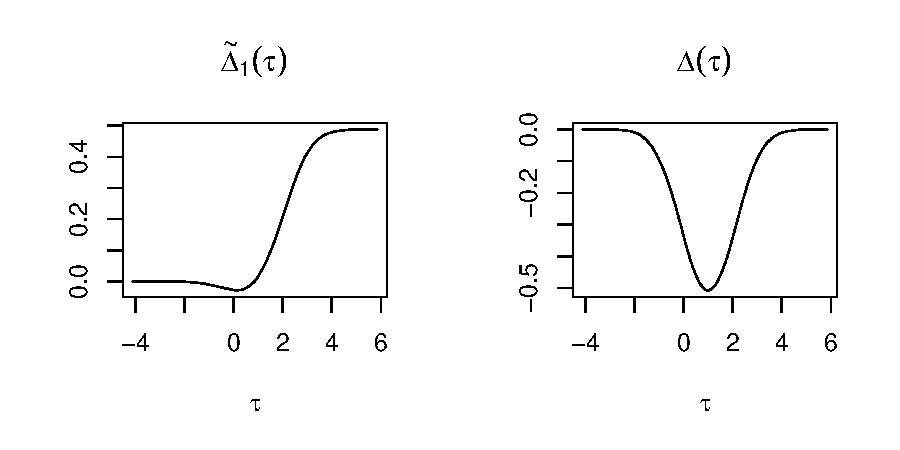
\includegraphics[width=\textwidth]{Delta_sim}
%  \end{figure}
%    
%    \vspace{-4em}
%\begin{align*}
%    \widetilde{\Delta}_1(\tau+\beta) - \widetilde{\Delta}_1(\tau) &= \alpha_0 \Delta(\tau + \beta) - (1 - \alpha_1) \Delta(\tau)\\
%  \Delta(\tau) &= F_k(\tau) - F_\ell(\tau)\\
%  \widetilde{\Delta}_1(\tau) &= p_k F_{1k}(\tau) - p_\ell F_{1\ell}(\tau)
%\end{align*}
%
%%  \end{block}
%
%  \normalsize
%\end{frame}
%%%%%%%%%%%%%%%%%%%%%%%%%%%%%%%%%%%%%
\begin{frame}
  \frametitle{Identification-Robust Joint Inference for $(\alpha_0, \alpha_1, \beta)$}
  \begin{itemize}
    \item Auxiliary moment inequalities to bound $(\alpha_0, \alpha_1)$
    \item Joint CS for $(\alpha_0, \alpha_1, \beta)$ by inverting Anderson-Rubin Test 
    \item Generalized Moment Selection (Andrews \& Soares, 2010) for tighter confidence sets.
  \end{itemize}
\end{frame}
%%%%%%%%%%%%%%%%%%%%%%%%%%%%%%%%%%%%%
\begin{frame}
  \begin{figure}
    \centering
    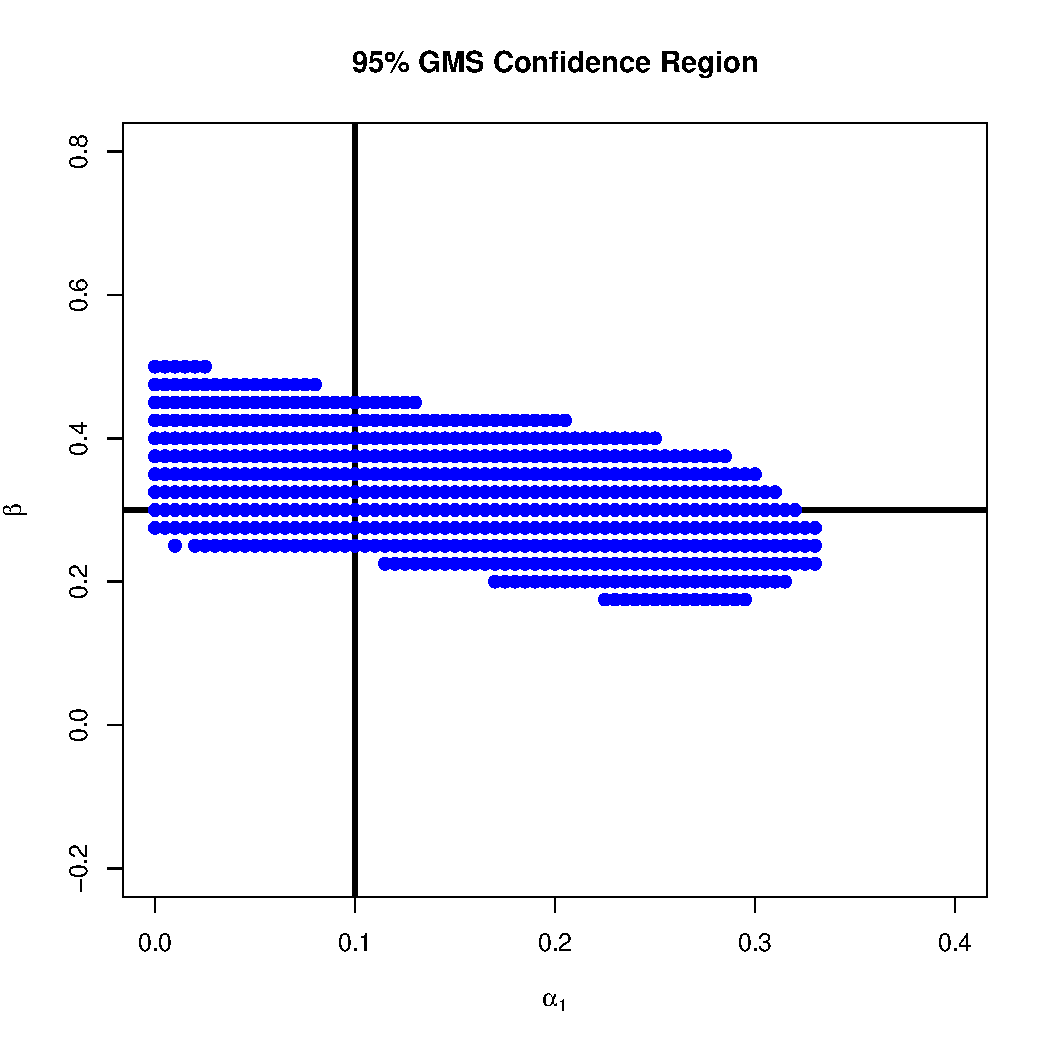
\includegraphics[scale=0.6]{GMS.pdf}
  \end{figure}
\end{frame}
%%%%%%%%%%%%%%%%%%%%%%%%%%%%%%%%%%%%%

\begin{frame}
  \frametitle{Conclusion}
  %\singlespacing
  %\small

  \begin{itemize}
    \item Endogenous, mis-measured binary treatment.
    \item Important in applied work but no solution in the literature.
      \item Usual (1st moment) IV assumption fails to identify $\beta$
      \item Higher moment / independence restrictions identify $\beta$
      \item Identification-Robust Inference incorportating additional inequality moment conditions.
   \end{itemize}

\end{frame}
%%%%%%%%%%%%%%%%%%%%%%%%%%%%%%%%%%%%%%%
\appendix

\begin{frame}[label=MAHAJAN_APPEND]
  \frametitle{Mahajan (2006, ECTA)}

  \vspace{-1em}

    \begin{columns}[c]
    \column{.45\textwidth} 
    \begin{exampleblock}{Regression Model}
      $y = \mathbb{E}[y|T^*] + \nu$\\
      {\small $\mathbb{E}[\nu|T^*]=0$ by construction}
    \end{exampleblock}
    \column{.45\textwidth}
    \begin{exampleblock}{Causal Model}
     $y = c + \beta T^* + \varepsilon$\\
     {\small$\mathbb{E}[\varepsilon|T^*]\neq 0$}
    \end{exampleblock}
    \end{columns}

    \vspace{1.5em}
  
  \begin{block}{Main Result (Correct) -- Exogenous Treatment}
   Relevant binary instrument $z$ ($p^*_k \neq p^*_\ell$) identifies $\alpha_0, \alpha_1$ and $\mathbb{E}[y|T^*]$ provided that $\mathbb{E}[\nu|T^*,T,z]=0$ and $\alpha_0 + \alpha_1 < 1$. 
  \end{block}

  \begin{alertblock}{Extension (Incorrect) -- Endogenous Treatment}
    $\mathbb{E}[\varepsilon|z]=0$, $p^*_k \neq p^*_\ell$, $\mathbb{E}[\varepsilon|T,T^*,z]=\mathbb{E}[\varepsilon|T^*] \implies$ $\beta$ identified.
  \end{alertblock}

\end{frame}

%%%%%%%%%%%%%%%%%%%%%%%%%%%%%%%%%%%%%%

\begin{frame}
  \frametitle{Mahajan (2006, ECTA)}
    \begin{columns}[c]
    \column{.45\textwidth} 
    \begin{exampleblock}{Regression Model}
      $y = \mathbb{E}[y|T^*] + \nu$\\
      {\small $\mathbb{E}[\nu|T^*]=0$ by construction}
    \end{exampleblock}
    \column{.45\textwidth}
    \begin{exampleblock}{Causal Model}
     $y = c + \beta T^* + \varepsilon$\\
     {\small$\mathbb{E}[\varepsilon|T^*]\neq 0$}
    \end{exampleblock}
    \end{columns}

    \vspace{0.7em}

    \begin{block}{Ingredients}
      
  \begin{enumerate}
    \item If $p^*_k \neq p^*_\ell$, $\mathbb{E}[\varepsilon|z]=0$ then, since $\beta_{IV} = \beta/(1-\alpha_0-\alpha_1)$, knowledge of $\alpha_0,\alpha_1$ is sufficient to recover $\beta$. \textcolor{blue}{(Correct)}
    \item If $p^*_k \neq p^*_\ell$, $\mathbb{E}[\nu|T^*,T,z]=0$, $\alpha_0, \alpha_1$ are identified. \textcolor{blue}{(Correct)}
    \item[] \alert{\framebox{How to satisfy both 1 and 2 while allowing $\mathbb{E}[\varepsilon|T^*]\neq 0$?}}
    \item[3.] Assume that $\mathbb{E}[\varepsilon|T^*,T,z]=\mathbb{E}[\varepsilon|T^*]$ \\ {\small (i.e.\ $m_{0k}^* = m_{0\ell}^*$ and $m_{1k}^*=m_{1\ell}^*$)}
  \end{enumerate}
    \end{block}
\end{frame}
%%%%%%%%%%%%%%%%%%%%%%%%%%%%%%%%%%%%%%
\begin{frame}
  \frametitle{Flaw in the Argument}
  \begin{block}{Proposition}
    If $\mathbb{E}[\varepsilon|T^*]\neq 0$ then  $\mathbb{E}[\varepsilon|T^*,T,z]=\mathbb{E}[\varepsilon|T^*]$ combined with $\mathbb{E}[\varepsilon|z]=0$ implies $p^*_k = p^*_\ell$, i.e.\ $z$ is irrelevant for $T^*$.
  \end{block}
  \begin{block}{Proof}
    $\mathbb{E}[\varepsilon|z]=0$ implies
  \begin{align*}
    (1-p_1^*) \textcolor{red}{m^*_{0k}} + p^*_1 \textcolor{blue}{m^*_{1k}}&=c\\
    (1-p_2^*) \textcolor{red}{m^*_{0\ell}} + p^*_2 \textcolor{blue}{m^*_{1\ell}}&=c
  \end{align*}
  while Mahajan's assumption implies $m_{0k}^* = m_{0\ell}^*$ and $m_{1k}^*=m_{1\ell}^*$.
  Therefore either $m_{0k}^*=m_{0\ell}^* = m_{1k}^* =m_{1\ell}^*=c$, which is ruled out by $E[\varepsilon|T^*]=0$, or $p^*_k = p^*_\ell$.
  \end{block}
    \hyperlink{MAHAJAN_BODY}{\beamergotobutton{Back}}
\end{frame}
%%%%%%%%%%%%%%%%%%%%%%%%%%%%%%%%%%%%%%%
\end{document}
